%*****************************************************
%	APPENDIX
%*****************************************************
\appendix
%-----------------------------------------------------
\chapter{Standard Quadrotor Dynamics}
\label{app:stddynamics}
%-----------------------------------------------------

%-----------------------------------------------------
\chapter{Design Bill of Materials}
\label{app:bom}
%-----------------------------------------------------
\section{Parts List}
%-----------------------------------------------------
\begin{table}[htbp]
\centering
\begin{tabularx}{\textwidth}{|X|l|l|}
\hline
\multicolumn{1}{|c|}{Part Name} & No. Used & Unit Weight[g]\\ \hline
\multicolumn{3}{|c|}{Electronics}\\ \hline
SPRacing F3 Deluxe Flight Controller & 1 & 6\\ \hline
OrangeRx 615X 2.4 GHz 6CH Receiver & 1 & 9.8\\ \hline
Signal Converter SBUS-PPM-PWM & 1 & 5.0\\ \hline 
STLink-V2 Debugger & 1 & N/A\\ \hline
RotorStar Super Mini S-BEC 10A & 1 & 30\\ \hline
128x96" OLED Display & 1 & N/A \\ \hline
XBee-Pro S1 & 2 & N/A \\ \hline
HobbyWing XRotor 15A Opto ESC & 4 & 10.5\\ \hline
OrangeRX RPM Sensor & 4 & 6\\ \hline
HobbyKing Multi-Rotor Power Distribution Board & 1 & 7.6\\ \hline
\multicolumn{3}{|c|}{Motors}\\ \hline
Corona DS-339MG & 8 & 32\\ \hline
Cobra 2208 2000KV Brushlesss DC & 4 & 44.2\\ \hline
\multicolumn{3}{|c|}{Frame Components}\\ \hline
APM Flight Controller Damping Platform & 1 & 16\\ \hline
HobbyKing SK450 Replacement Arm (2 pcs) & 2 & N/A\\ \hline
SK450 Extended Landing Skid & 1 & 93\\ \hline
Alloy Servo Arm (FUTABA) & 8 & N/A\\ \hline
10X18X6 Radial Ball Bearing & 8 & N/A\\ \hline
80g Damping Ball & 32 & N/A\\ \hline
Plastic Retainers for Damping Balls & 32 & N/A\\ \hline
3/5mm Aluminum Prop Adapter & 4 & N/A\\ \hline
6x4.5 Gemfam 3-Blade Propeller & 4 & N/A\\ \hline
M3 6mm Hex Nylon Spacer & 8 & N/A\\ \hline
M3 16mm Hex Nylon Spacer & 32 & N/A\\ \hline
M3 25mm Nylon Screw & 128 & N/A\\ \hline
M2.5x10mm Socket Head Cap Screw & 36 & N/A\\ \hline
M2.5x25mm Socket Head Cap Screw & 20 & N/A\\ \hline
M2.5 A-Lok Nut & 16 & N/A\\ \hline 
\end{tabularx}
\label{tab:partslist}
\caption{Parts List}
\end{table}
%-----------------------------------------------------
\newpage
%-----------------------------------------------------
\newgeometry{left=1cm,right=1cm,top=2cm,bottom=2cm}
\begin{figure}[hbtp]
\vspace{-20pt}
\centering
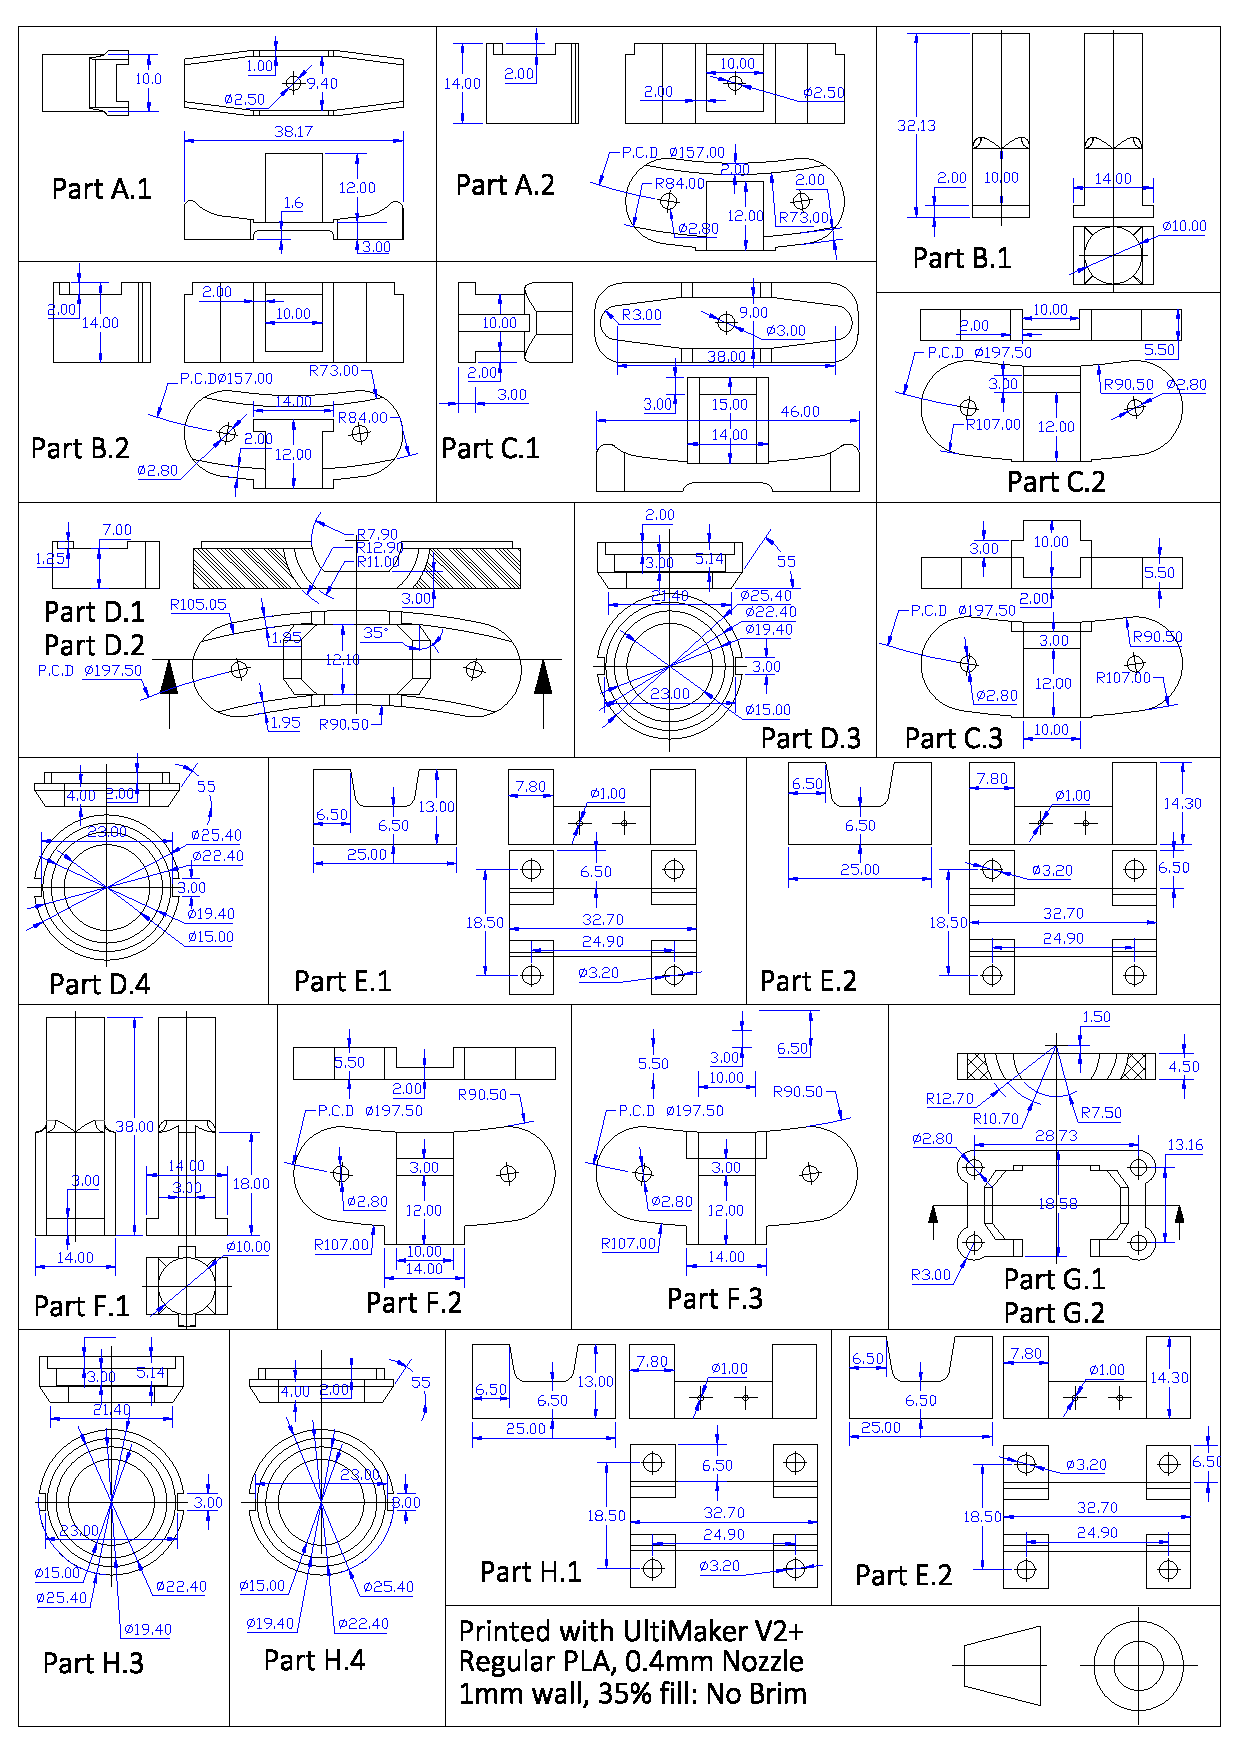
\includegraphics[width=\textwidth]{pdfpages/working.pdf}
\captionof{table}{3D Printed Parts}
\end{figure}
\restoregeometry
%-----------------------------------------------------
\newpage
%-----------------------------------------------------
\newgeometry{left=1cm,right=1cm,top=2cm,bottom=1cm}
\begin{table}[htbp]
\label{tab:damping-assemblies}
\centering
\begin{tabularx}{\textwidth}{|X|X|}
\hline
\multicolumn{2}{|c|}{Bracket Assemblies 2}\\
\hline
\begin{minipage}{0.5\textwidth}
\vspace{6pt}
\centering
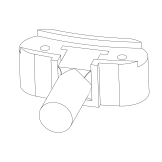
\includegraphics[width=0.7\textwidth]{figs/appendix/assembly-inner-bearing}
\captionof{figure}{Bearing Bracket Inner Ring Assembly}
Parts: A.1, A.2
\end{minipage}
&
\begin{minipage}{0.5\textwidth}
\vspace{6pt}
\centering
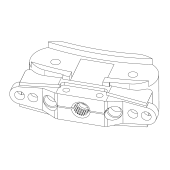
\includegraphics[width=0.7\textwidth]{figs/appendix/assembly-inner-servo}
\captionof{figure}{Servo Bracket Inner Ring Assembly}
Parts: B.1, B.2, M3 Servo Horn
\end{minipage}
\\
\hline
\begin{minipage}{0.5\textwidth}
\vspace{6pt}
\centering
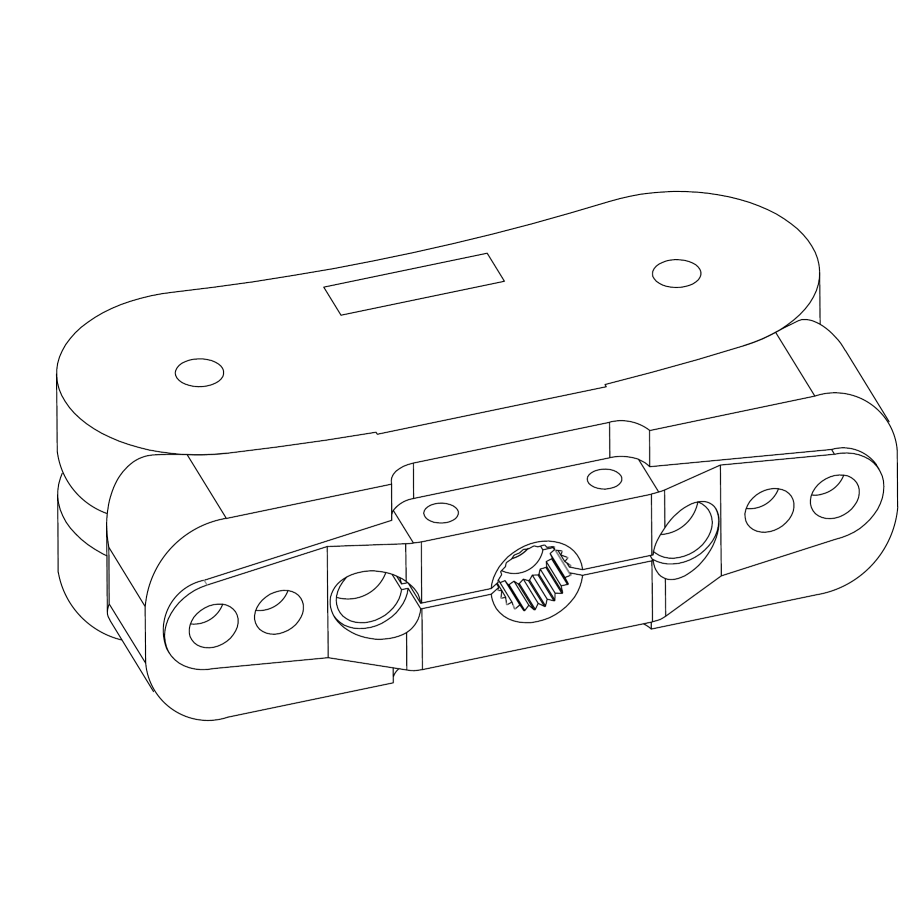
\includegraphics[width=0.7\textwidth]{figs/appendix/assembly-middle-servo-bracket}
\captionof{figure}{Servo Bracket Middle Ring Assembly}
Parts: C.1, C.2, C.3, M3 Servo Horn
\end{minipage}
&
\begin{minipage}{0.5\textwidth}
\vspace{6pt}
\centering
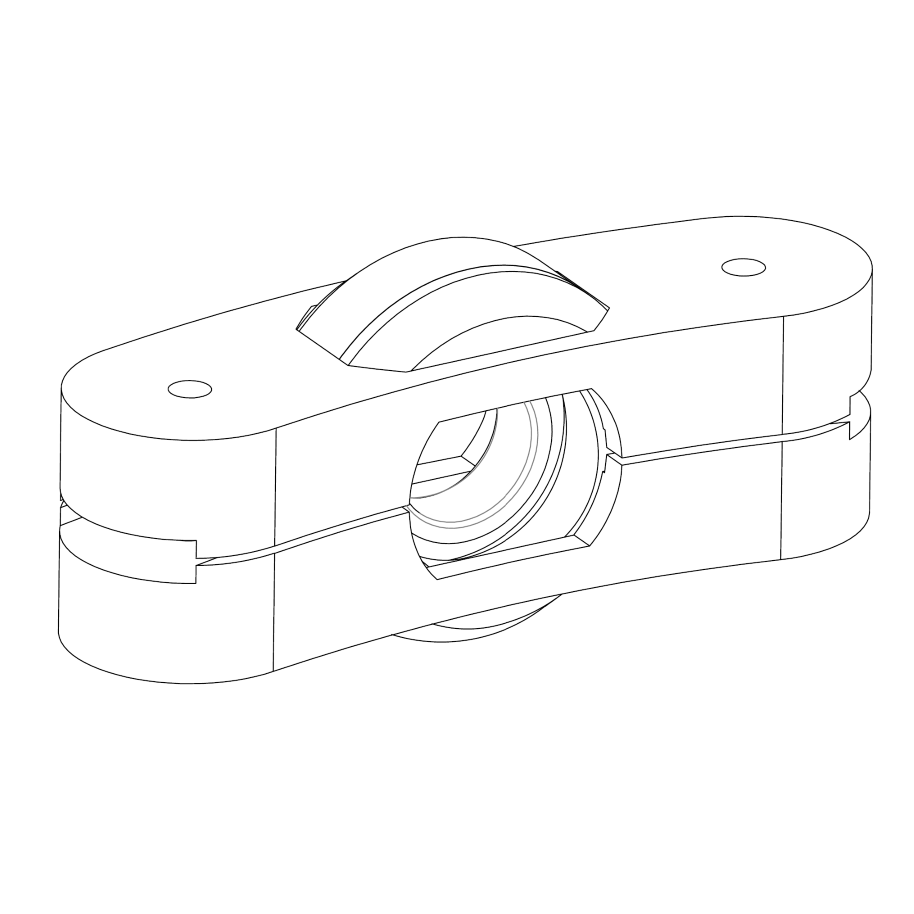
\includegraphics[width=0.7\textwidth]{figs/appendix/assembly-middle-bearing-holder}
\captionof{figure}{Bearing Holder Middle Ring Assembly}
Parts: D.1, D.2, D.3, D.4, 18-10 Bearing
\end{minipage}
\\
\hline
\begin{minipage}{0.5\textwidth}
\vspace{6pt}
\centering
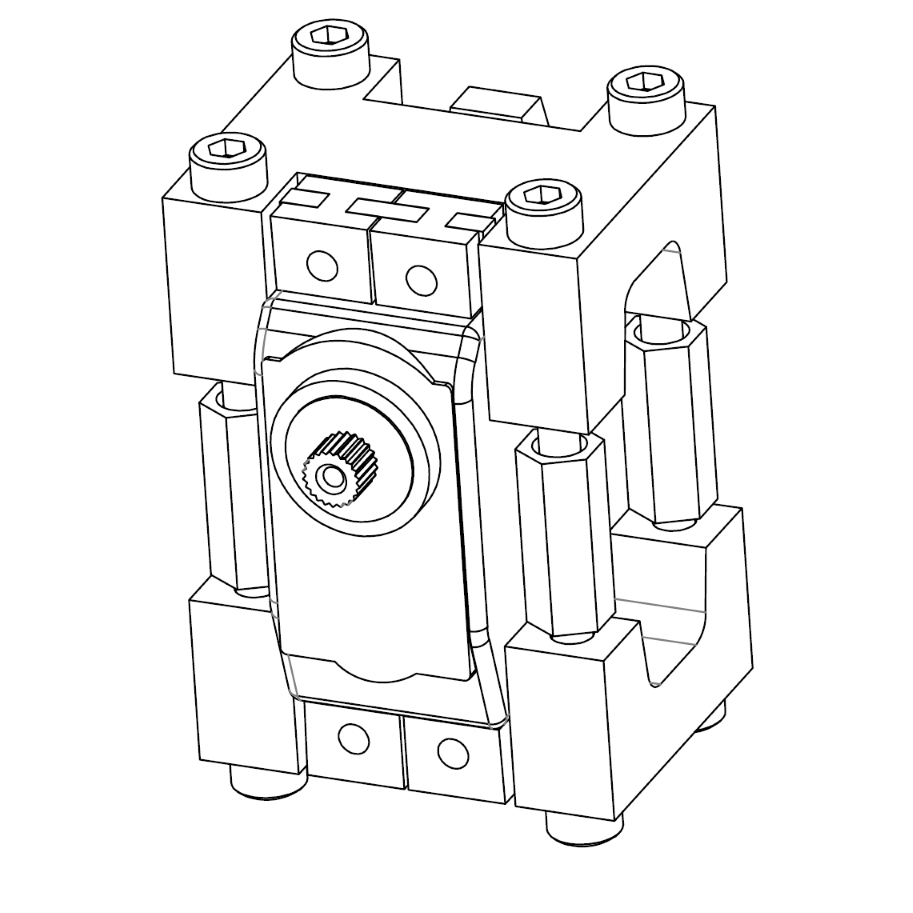
\includegraphics[width=0.7\textwidth]{figs/appendix/assembly-middle-servo-mount}
\captionof{figure}{Servo Mount Middle Ring Assembly}
Parts: E.1, E.2, Corona Servo \& Fasteners
\end{minipage}
&
\begin{minipage}{0.5\textwidth}
\vspace{6pt}
\centering
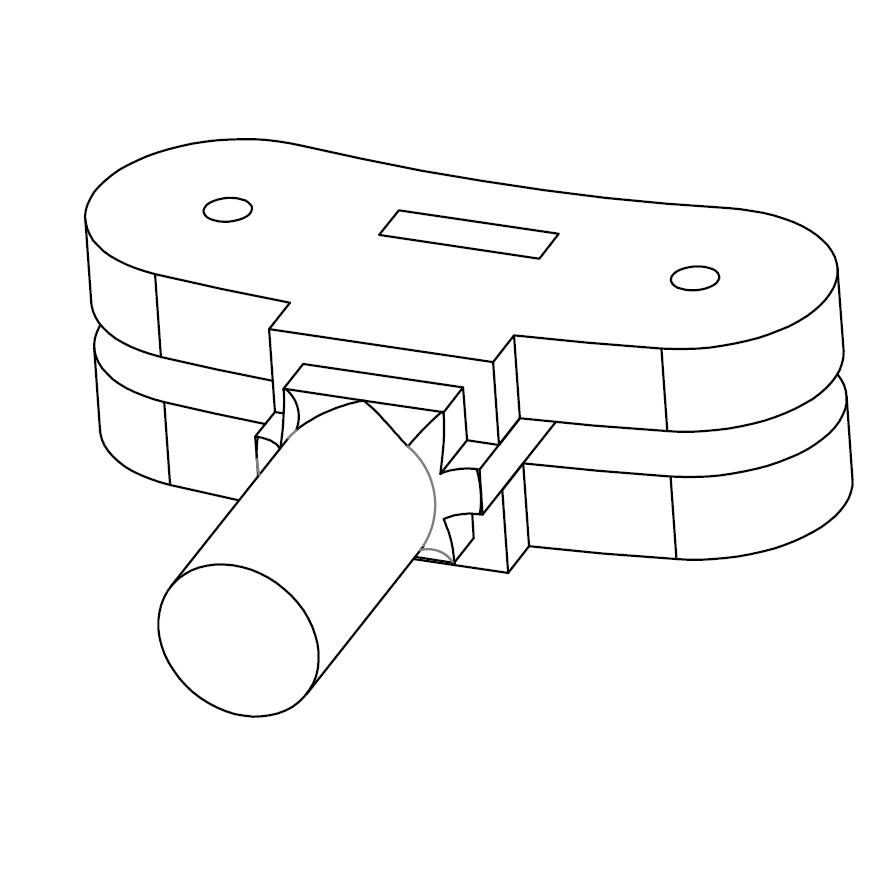
\includegraphics[width=0.7\textwidth]{figs/appendix/assembly-middle-bearing-bracket}
\captionof{figure}{Bearing Shaft Middle Ring Assembly}
Parts: F.1, F.2, F.3
\end{minipage}
\\
\hline
\end{tabularx}
\caption{Inner \& Middle Ring Assemblies}
\end{table}
\restoregeometry
%-----------------------------------------------------
\newpage
%-----------------------------------------------------
% Table 2
\newgeometry{left=1cm,right=1cm,top=2cm,bottom=0.5cm}
\begin{table}[htbp]
\label{tab:damping-assemblies}
\centering
\begin{tabularx}{\textwidth}{|X|X|}
\hline
\multicolumn{2}{|c|}{Bracket Assemblies 2}\\
\hline
\begin{minipage}{0.5\textwidth}
\vspace{6pt}
\centering
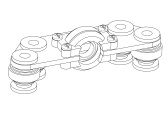
\includegraphics[width=0.7\textwidth]{figs/appendix/assembly-damping-bearing}
\captionof{figure}{Bearing Holder Damping Assembly}
Parts: G.1, G.2, G.3, G.4, 18-10 Bearing, 80g 
\\
Damping Balls, Bearing Holder Damping Bracket
\end{minipage}
&
\begin{minipage}{0.5\textwidth}
\vspace{6pt}
\centering
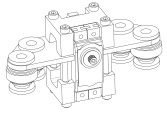
\includegraphics[width=0.7\textwidth]{figs/appendix/assembly-damping-servo}
\captionof{figure}{Servo Mount Damping Assembly}
Parts: H.1, H.2, Corona Servo \& Fasteners, 80g Damping Balls, Servo Mount Damping Bracket
\end{minipage}
\\
\hline
\end{tabularx}
\caption{Damping Assemblies}
\end{table}
\par
\begin{table}[htbp]
\label{tab:damping-backets}
\centering
\begin{tabularx}{\textwidth}{|X|X|}
\hline
\multicolumn{2}{|c|}{Laser Cut Brackets}\\
\hline
\begin{minipage}{0.5\textwidth}
\vspace{6pt}
\centering
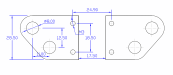
\includegraphics[width=0.8\textwidth]{figs/appendix/damping-bracket-servo}
\captionof{figure}{Servo Mount Damping Bracket}
\end{minipage}
&
\begin{minipage}{0.5\textwidth}
\vspace{6pt}
\centering
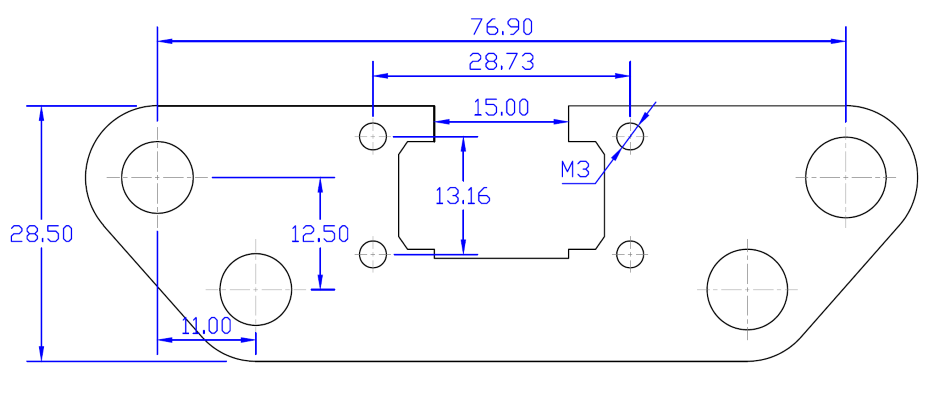
\includegraphics[width=0.8\textwidth]{figs/appendix/damping-bracket-bearing}
\captionof{figure}{Bearing Holder Damping Bracket}
\end{minipage}
\\
\hline
\begin{minipage}{0.5\textwidth}
\vspace{12pt}
\centering
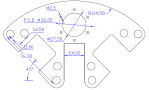
\includegraphics[width=0.9\textwidth]{figs/appendix/damping-arm-mount}
\captionof{figure}{Arm Mount Damping Bracket}
\end{minipage}
&
\begin{minipage}{0.5\textwidth}
\vspace{6pt}
\centering
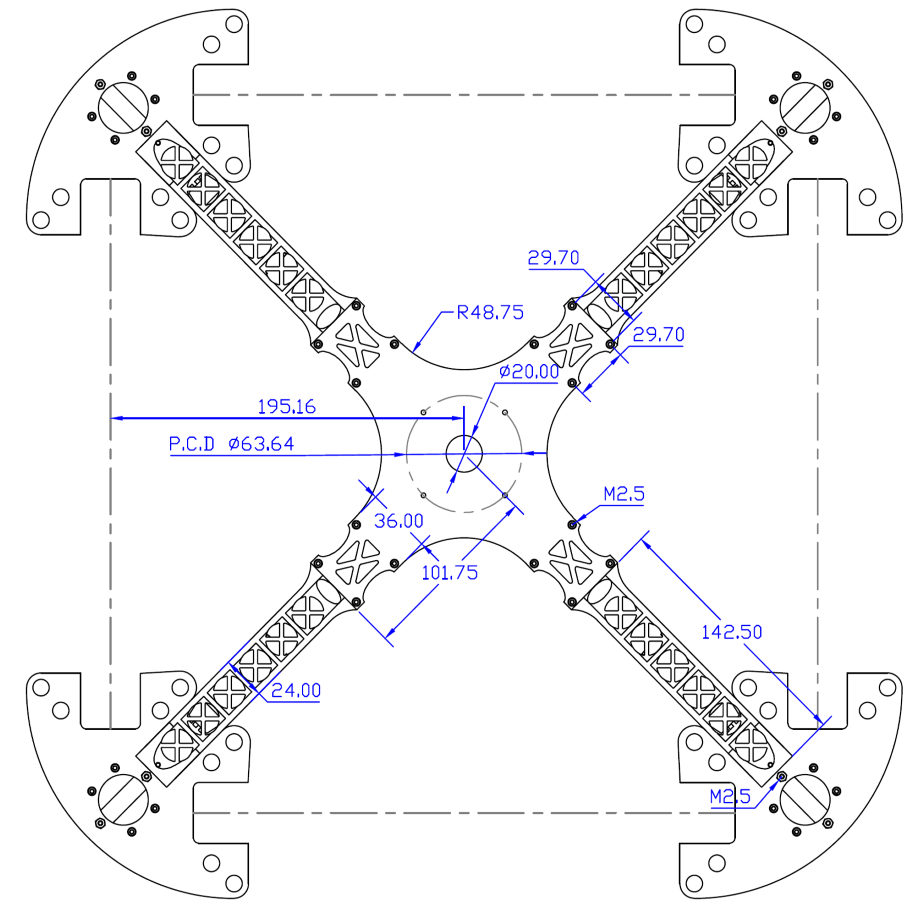
\includegraphics[width=0.6\textwidth]{figs/appendix/frame-assembly}
\captionof{figure}{Frame Brackets}
\end{minipage}
\\
\hline
\end{tabularx}
\caption{Laser Cut Damping Brackets}
\end{table}

\restoregeometry
%-----------------------------------------------------
\newpage
%-----------------------------------------------------
\newgeometry{left=1cm,right=1cm,top=2cm,bottom=1cm}
\vspace{-20pt}
\begin{figure}[hbtp]
\centering
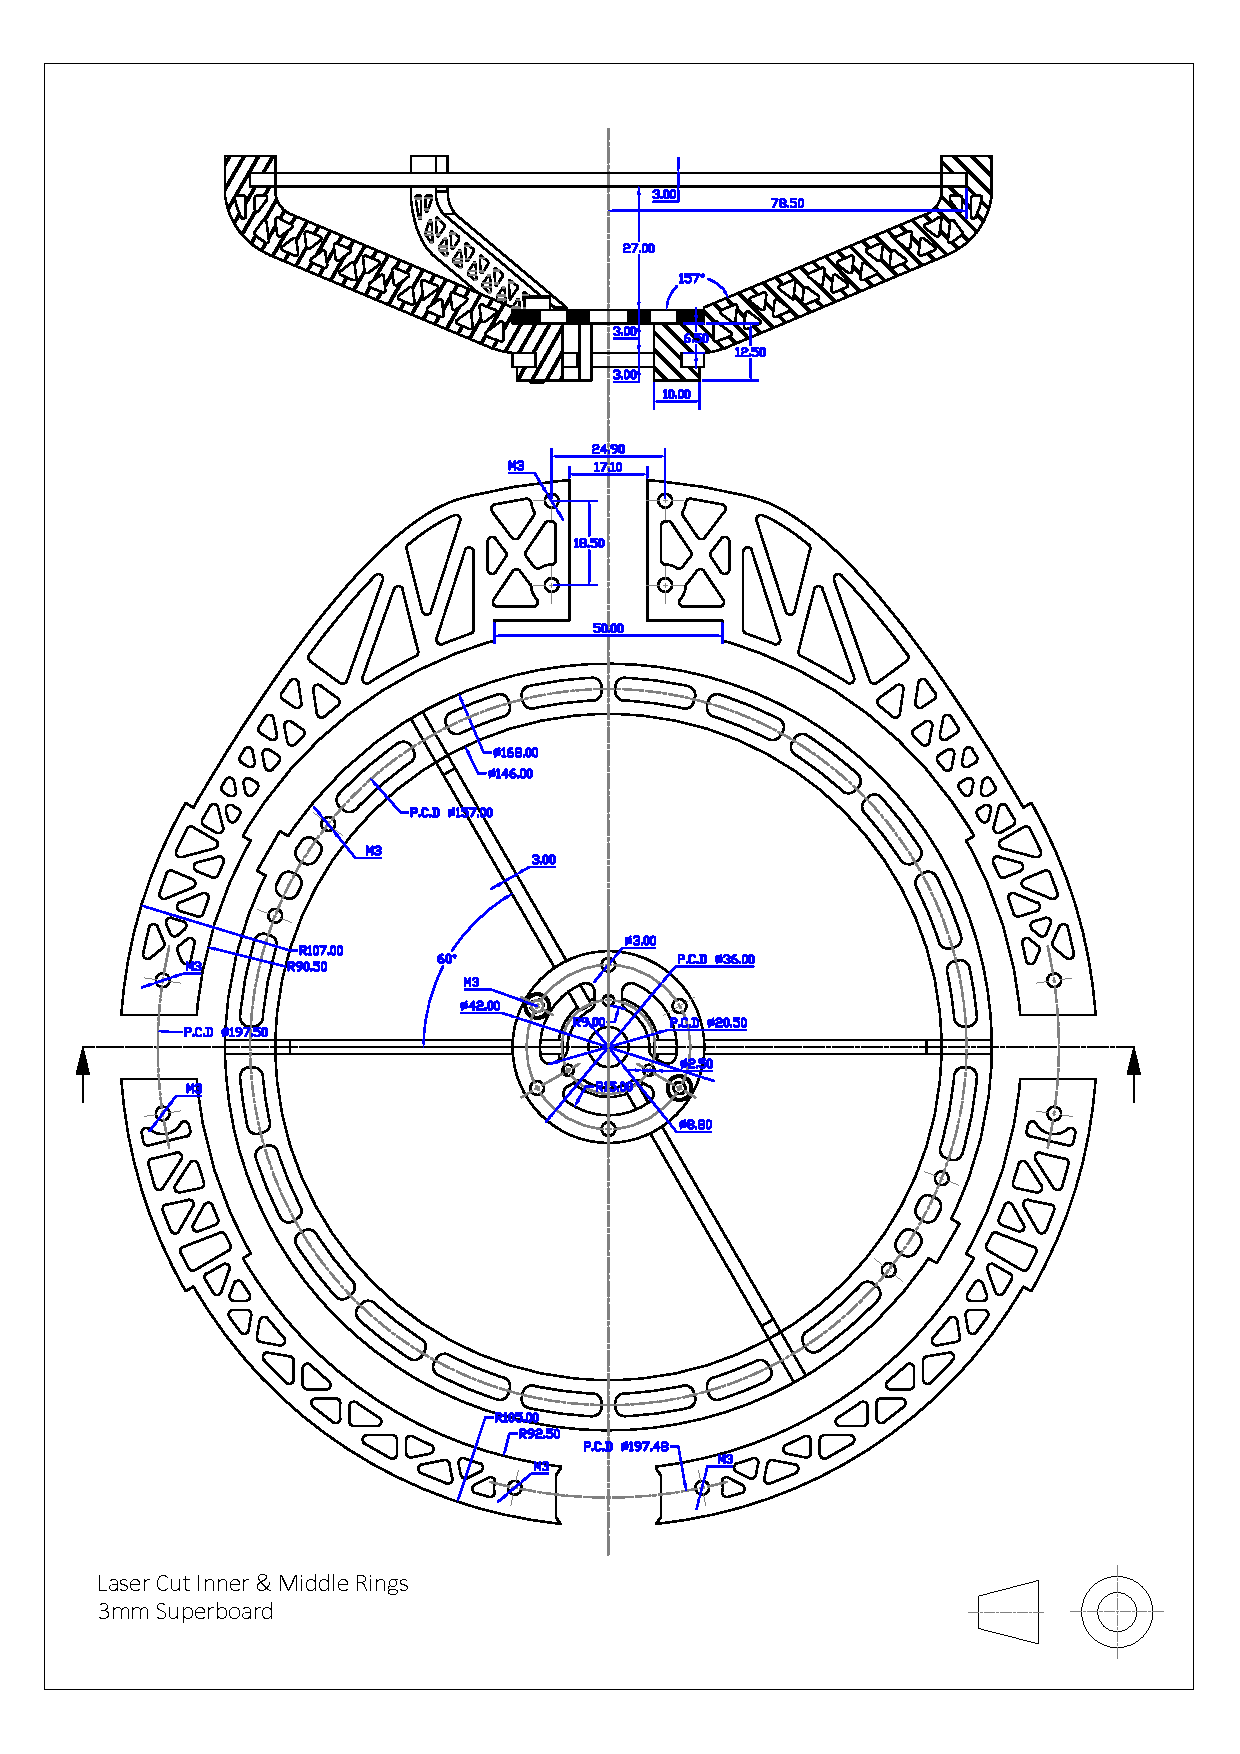
\includegraphics[width=0.95\textwidth]{pdfpages/rings.pdf}
\captionof{table}{Laser Cut Parts}
\end{figure}
\restoregeometry
%-----------------------------------------------------
\newpage
%-----------------------------------------------------
\newgeometry{left=1cm,right=1cm,top=2cm,bottom=1cm}
\section{F3 Deluxe Schematic Diagram}
\label{app:deluxe-diagram}
{\centering
\fbox{
\begin{minipage}{0.9\textwidth}
\centering
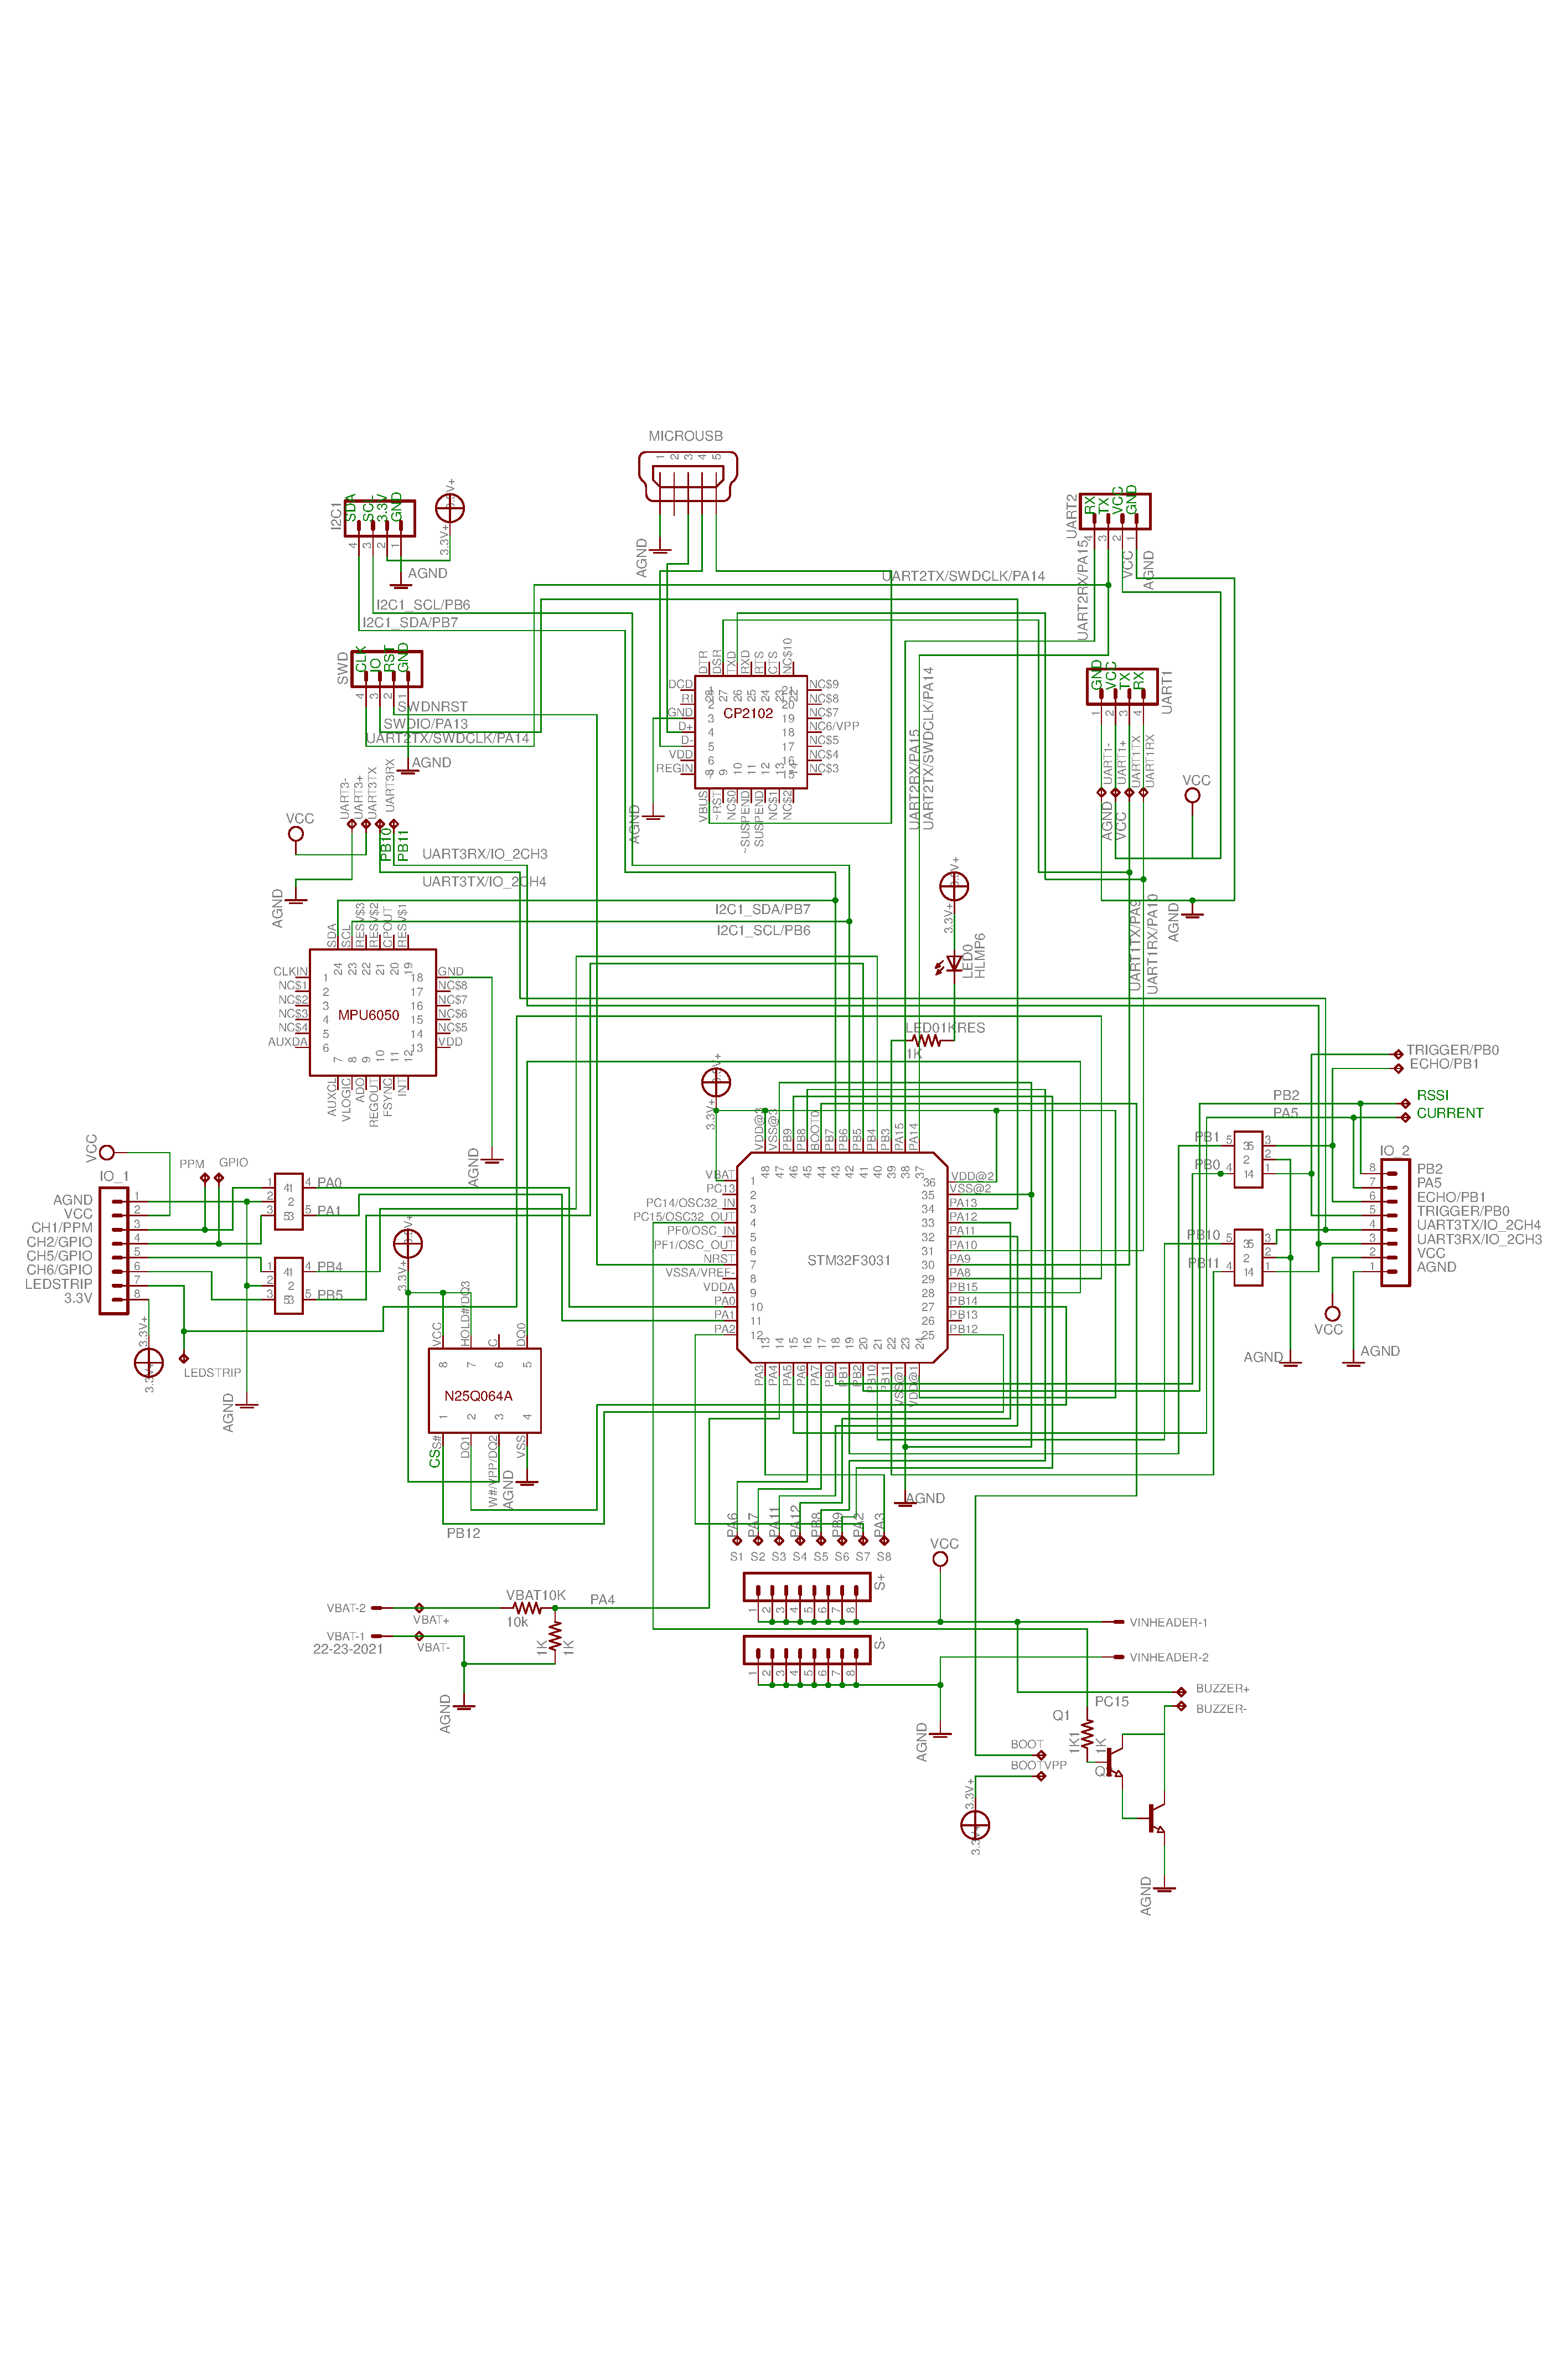
\includegraphics[width=0.9\textwidth]{pdfpages/deluxe-schematic.pdf}
\end{minipage}
}
\captionof{figure}{F3 Deluxe Flight Controller Hardware Schematic}
}
\restoregeometry
%-----------------------------------------------------
\newpage
%-----------------------------------------------------
\chapter{System ID Test Data}
\label{app:systemdat}
%-----------------------------------------------------
\section{Servo Data}
%-----------------------------------------------------
\newpage
%-----------------------------------------------------
\newgeometry{left=1cm,right=1cm,top=2cm,bottom=1cm}
\section{Cobra CM2208-200KV}
\label{app:cobra-test}
\centering
\fbox{
\begin{minipage}{0.9\textwidth}
\centering
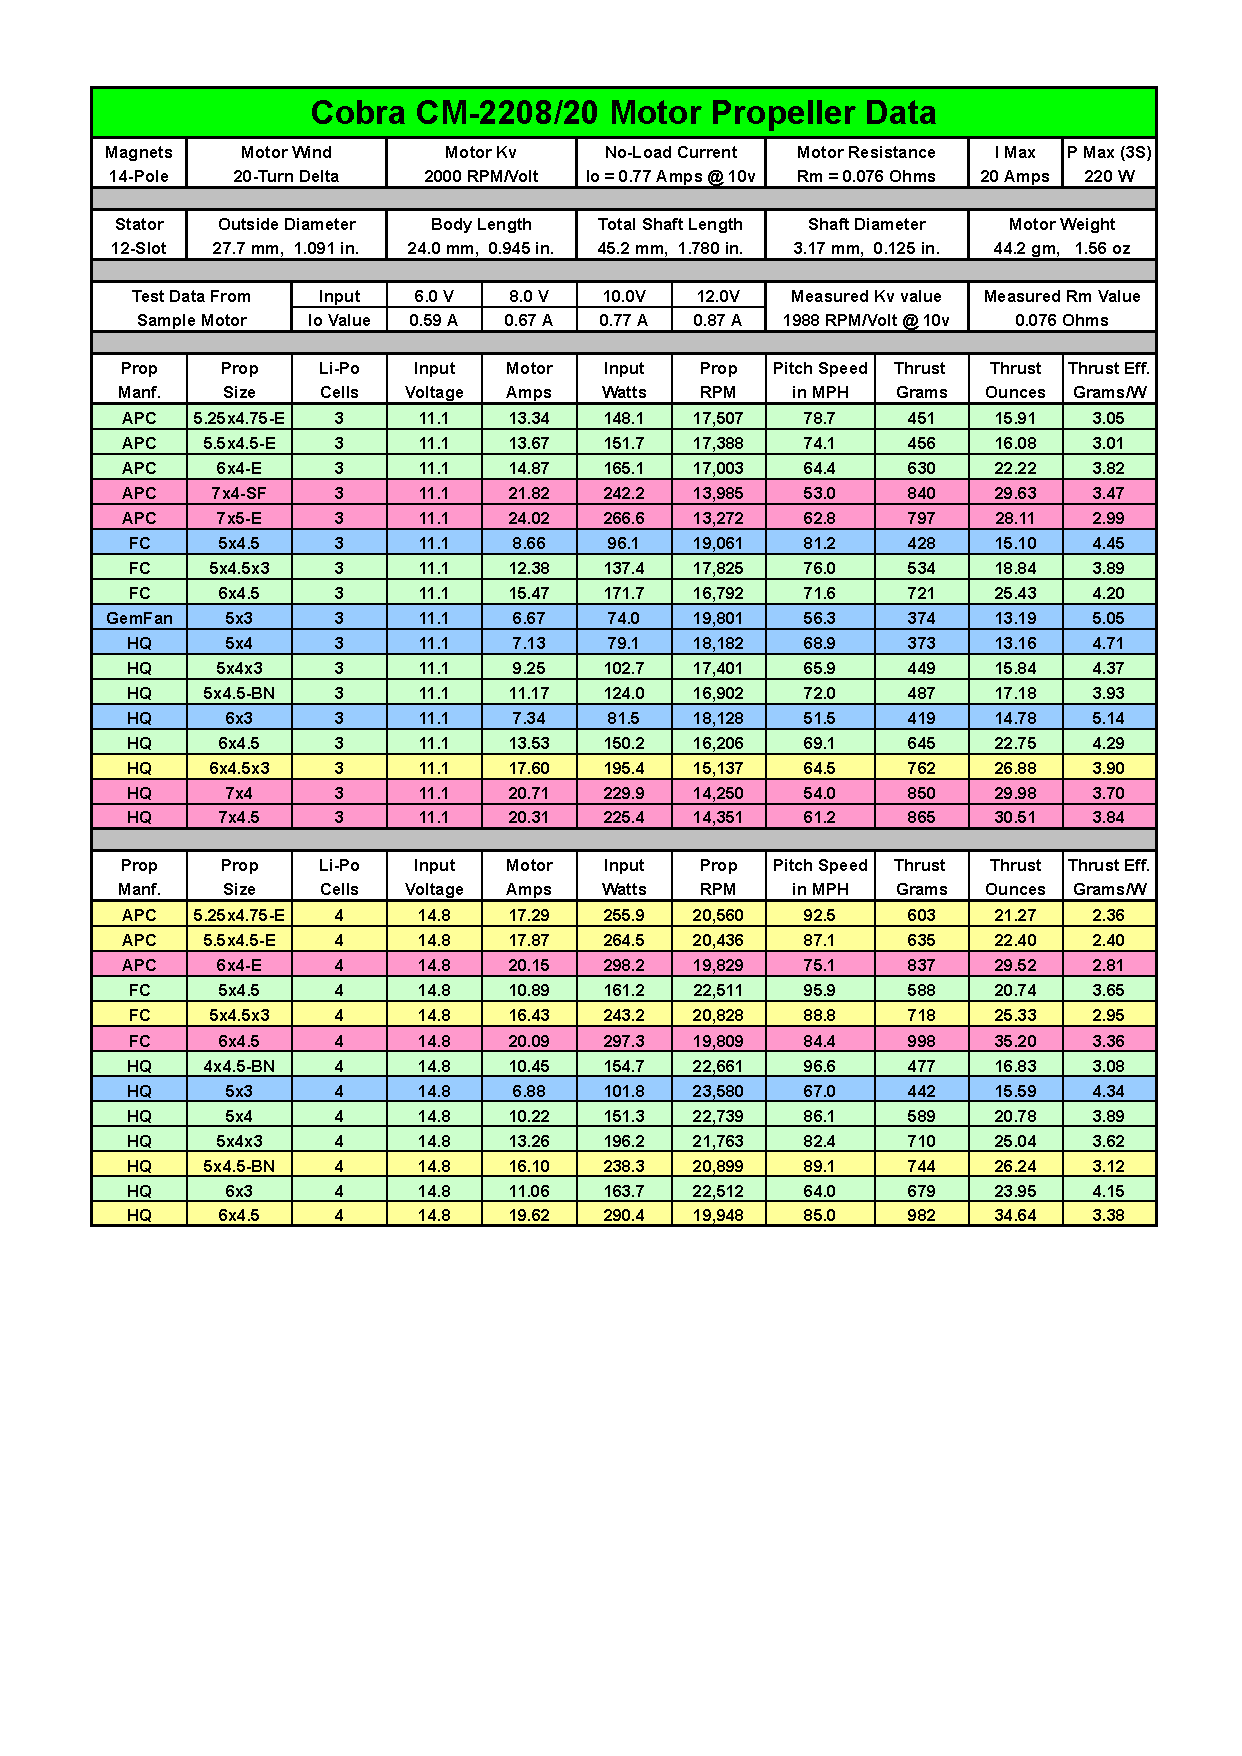
\includegraphics[width=\textwidth]{pdfpages/cobra-test.pdf}
\end{minipage}
}
\captionof{figure}{Official Test Results for Cobra Motors}
\restoregeometry
%-----------------------------------------------------
\newpage
%-----------------------------------------------------
\chapter{Full Equations}
\label{app:eq}
\section{Inertias}
\begin{subequations}
\begin{equation} \label{eq:app.inertia}
\approx\begin{bmatrix}
3613.144 & 0.025 & 406.81\\
0.025 & 9774.160 & 0.4626\\
406.81 & 0.4626 & 12650.72\\
\end{bmatrix}
\end{equation}
\vspace{-5pt}
\begin{equation}
\begin{bmatrix}
0 & -0.249s\lambda-0.276c\lambda & 0.249c\lambda-0.276s\lambda\\
-0.249s\lambda-0.276c\lambda & -0.448s2\lambda -2142.67s\lambda+983c\lambda&983s2\lambda-2142.67s\lambda+0.448c2\lambda\\
0.249c\lambda-0.276s\lambda & 983s2\lambda -2142.67s\lambda +0.448c2\lambda & 1967.497s\lambda + 1070.88c2\lambda+0.448s2\lambda\\
\end{bmatrix}
\end{equation}
\begin{equation}
=\begin{bmatrix}
814c_{\eta}s_{\eta} + 3613{c^2}_{\eta} + 11580{s^2}_{\eta} + 2142{c^2}_{\lambda}{s^2}_{\eta} + 1967{s^2}_{\eta}{s^2}_{\lambda} + 2c_{\lambda}{s^2}_{\eta}s_{\lambda} - c_{\eta}s_{\eta}s_{\lambda}
\\
2{c^2}_{\lambda}s_{\lambda} - s_{\lambda} - 175c_{\lambda}s_{\eta}s_{\lambda}
\\
4967s_{2\eta} + 814{c^2}_{\eta} - {c^2}_{\eta}s_{\lambda} + 175c_{\eta}{c^2}_{\lambda}s_{\eta} + 2c_{\eta}c_{\lambda}s_{\eta}s_{\lambda}
\\
2{c^2}_{\lambda}s_{\eta} - s_{\eta} - 175c_{\lambda}s_{\eta}s_{\lambda}
\\
10933 - 175{c^2}_{\lambda} - s_{2\lambda}
\\
2c_{\eta}{c^2}_{\lambda} - c_{\eta} - 175c_{\eta}c_{\lambda}s_{\lambda}
\\
4967s_{2\eta} + 814{c^2}_{\eta} - {c^2}_{\eta}s_{\lambda} + 175c_{\eta}{c^2}_{\lambda}s_{\eta} + 2c_{\eta}c_{\lambda}s_{\eta}s_{\lambda} - 407
\\
2c_{\eta}{c^2}_{\lambda} - c_{\eta} - 175c_{\eta}c_{\lambda}s_{\lambda}
\\
9933{c^2}_{\eta} - 814c_{\eta}s_{\eta} + 175{c^2}_{\eta}{c^2}_{\lambda} + 2{c^2}_{\eta}c_{\lambda}s_{\lambda} + c_{\eta}s_{\eta}s_{\lambda}
\end{bmatrix} 
\end{equation}
\vspace{-10pt}
\begin{equation}
=\mathbb{R}_Z
\begin{bmatrix}
c_{\eta_i} & 0 & s_{\eta_i}\\
0 & 1 & 0\\
-s_{\eta_i} & 0 & c_{\eta_i}\\
\end{bmatrix}\big(
\mathbb{I}_{M_i'}\big)
\begin{bmatrix}
c_{\eta_i} & 0 & -s_{\eta_i}\\
0 & 1 & 0\\
s_{\eta_i} & 0 & c_{\eta_i}\\
\end{bmatrix}
\mathbb{R}_Z^{-1}
\end{equation}
\end{subequations}
